\chapter{Introduction}
\section{e-Government and e-Governance}
% The words `e-government' and `e-governance' are used interchangeably, most often due to lack of dissemination of authentic information on these subjects. The difference between the two has been succinctly brought out by ~{Mr. Thomas B. Riley}.\par

% \begin{quotation}
% 	\noindent Government and governance are both about getting the consent and cooperation of the governed. But whereas governmnet is the formal apparatus for this objective, governance is the outcome as experienced by those on the receiving end. e-government can be more productive version of government in general, if it is wll implemented and managed. e-governance can evolve into participatory governance if it is well supported with the appropriate principles, objective, programs and architectures.
% \end{quotation}



% e-governance is the modernization of processes and functions of the government using the tools of ICT so as to transform the way it servers its constituents. Citizens are seen here as ``passive recipients'' of digital information and services.

% e-governance, on the other hand, is seen as a `decisional process'. It is about the use of ICT in systems of governance so as to ensure a wider participation and deeper involvement of citizens, institutions, NGOs and companies, in the decision-making process of governance - wider and deeper than is possible in the conventional forms and forums of consulation in democracies today.

% \begin{quotation}
% 	\noindent e-governance is beyond the scope of e-government. While e-government is defined as a mere delivery of government services and information to the public using electronic means, e-governance allows direct participation of constituents in government activities \(\ldots\)[e-governance] will bring forth new concepts of citizenship both in terms of needs and responsibilities.
% \end{quotation}

e-government is the process of transformation of the relationships of government with its constituents - the citizens, the businesses - and between its own organs, through the use of the tools of ICT, the aim is to bring about enhanced access, transparency, accountability and efficiency in the delivery of government information and services.

Government exist for the people and for the businesses that people are engaged in. The mandate of any democratic government is to provide a set of services in an efficient, convenient, equitable and cost-effective manner so as to ensure the welfare and well being of its citizens and to facilitate the growth of economic activities. An epithet that has gained popularity in this context is \textit{SMART government}, that is:
\begin{multicols}{3}
	\begin{itemize}
		\item \textbf{S}imple
		\item \textbf{M}oral
		\item \textbf{A}ccountable
		\item \textbf{R}esponsive and
		\item \textbf{T}ransparent
	\end{itemize}
\end{multicols}

Essentially, \textit{SMART} captures all the important attributes of good governance.


\begin{framed}
	\begin{nepali}
		\noindent e-Governance का ५ सिद्धान्तहरु / five principles of  e-governance भनेर यही 'SMART' लाई पनि भनिन्छ।
	\end{nepali}
\end{framed}

\subsection*{Simple}
\textit{Simple} would mean simplicity of the laws, rules, regulations, processed and procedures of government.

\subsection*{Moral}
\textit{Moral} government mean emergence of an entirely new system of ethical values in the polictical and administrative machinery.

\subsection*{Accountability}
\textit{Accountability} raises the question: \textit{who is accountable to whom and in what way?}

\subsection*{Responsiveness}
\textit{Responsiveness} in the context of good governance, means to be alive to the needs of the public and to exhibit the required degree of urgency in responding to such needs. It includes quality of service and its timeliness. 

An important concept developed in this context is the \textbf{Citizen Charter}. Citizen Charters are a set of assurances given by government agencies on the quality of services and the time limit for their delivery.

\subsection*{Transparency}
\textit{Transparency} basically arises out of the citizen's right to information - the right to know what decisions public institutions take and for what valid reasons. The publication of such information should be up-to-date and logically ordered for easy access.

Examles: 

	\begin{itemize}
		\item assessment of taxes payable by citizens and businesses
		\item appointments to public posts
		\item disciplinary matters of employees
		\item selection of beneficiaries for social welfare schemes
		\item grant of concessions to private sector in public-private partnership scenario, and 
		\item allocation of scarce resources among competing demands
	\end{itemize}
	


%TODO: e-government र e-governance काे सम्पादन बाँकी
\subsection{e-Government}
%https://publicadministration.un.org/egovkb/en-us/about/unegovdd-framework
E-government has been employed to mean everything from \textit{online government services} to \textit{exchange of information and services electronically with citizens, businesses, and other arms of government}. Traditionally, e-government has been considered as the use of ICTs for improving the efficiency of government agencies and providing government services online. Later, the framework of e-government has broadened to include use of ICT by government for conducting a wide range of interactions with citizens and businesses as well as open government data and use of ICTs to enable innovation in governance.\par

E-government can thus be defined as \textit{the use of ICTs to more effectively and efficiently deliver government services to citizens and businesses}. It is the application of ICT in government operations, achieving public ends by digital means. The underlying principle of e-government, supported by an effective e-governance institutional framework, is to improve the internal workings of the public sector by reducing financial costs and transaction times so as to better integrate work flows and processes and enable effective resource utilization across the various public sector agencies aiming for sustainable solutions. Through innovation and e-government, governments around the world can be more efficient, provide better services, respond to the demands of citizens for transparency and accountability, be more inclusive and thus restore the trust of citizens in their governments.


\subsection{e-Governance}
E-Governance is a form of e-business in governance comprising of processes and structures
involved in deliverance of electronic services to the public, viz. citizens. It also involves
collaborating with business partners of the government by conducting electronic transactions
with them. Besides, it entails enabling the general public to interact with the government,
through electronic means, for getting the desired services. In other words, e-governance
means application of electronic means in the interaction between.

\begin{itemize}
	\item government (G) and citizens (C), both ways (i.\ e.\ G2C, and C2G),
	\item government or business (B), both ways (i.\ e.\ G2B and B2G), and
	\item internal government operation (G2G)
\end{itemize}

The aim, ultimately, is to simplify and improve governance and enable people's participation in
governance through mail, and Internet.

E-governance is much more than just preparing some websites. It ranges from the use of
Internet for dissemination of plain web based information at its simplest level to services and
online transactions on the one hand and utilizing IT in the democratic process itself, i.\ e.\
election on the other.

e-governance implies e-democracy, wherein all forms of interaction between the electorate
(i.\ e.\ general public) and the elected (i.\ e.\ the government) are performed electronically. e-government, as distinguished from e-governance, comprises a pragmatic application and
usage of the most innovative technologies in computer and communication technologies,
including Internet technology, for delivering efficient and cost effective services, and
Information and knowledge to the citizens being governed, thereby realizing the vast potential
of the government to serve the citizens.

Various manifestations of e-governance initiative will be in terms of the government delivering
services to citizens of transacting business, offering general information, or conducting
interactions with the general public and business using such IT tools as:
\begin{itemize}
	\item E-mail
	\item Internet websites publishing (including online interactive transaction)
	\item WAP application and publishing
	\item SMS connectivity
	\item Intranet development and usage
	\item Promotion of citizen access.
\end{itemize}

The advent of these other components and of Information and Communication Technology
(ICT) as a highly leveraged enabling tool for delivery of services in the public and private sector has now been universally recognized. This has resulted in a redefinition of the fundamental concept of governance and also in recognizing its potential to change both institutions and delivery mechanisms of services for betterment of people.

%\subsection*{Need for e-Governance}
%The fundamental motivation for the campaign is a slogan—to provide SMART government—``SMART" being an acronym for Simple, Moral,
%Accountable, Responsive and Transparent Government, a laudable ideal, though difficult it
%may be to achieve in reality. Thus, we may conceive a Smart Village or Smart Municipality or
%Smart State, all very difficult but ideal models. Notwithstanding the difficulties involved in
%achieving this, a clear objective of e-governance can be cutting the cost of e-governance and
%also minimizing the complexities of the procedures by possible business process
%re-engineering. The concomitant benefit is empowerment of people through what is called
%`disintermediation'; in other words, eliminating the middleman or tout between the
%government and the people. For example, by doing so, property tax assessment and collection
%system can reduce the element of corruption in the system apart from increasing consumer
%convenience. The online system based on the Internet will reduce contacting with the
%mediating officials, thereby reducing the possibility of malpractice. This does not however
%mean that the primary objective of e-governance is tackling with corruption, even though it
%may be a fallout (though not necessarily).
%
%Evidently, the objectives of achieving such e-governance go far beyond mere simple
%computerization of stand-alone back office operations in government offices. It should mean a
%drastic change in the way the government operates, and this means a new and redefined set
%of responsibilities for the executive, legislative and the judiciary. This requires bringing about a
%social catharsis, which needs to be done in a comprehensive, concerted and planned manner.
%
%Historically, it was Chile that a real e-governance initiative was taken up as early as in 1972,
%when the IT applications were unheard of in government and were limited even in the
%business. They used techniques of IT not to just make government paperless or less of paper
%(as is presently being done) but to perform government work efficiently. They realized that
%transparency is the ability to regulate the conditions, not the transactions. Prof. Stafford Beer
%implemented for President Allende of Chile, the first e-governance software that would help
%the government survive a severe crisis. The question that was asked to and answered by the
%software was whether the government would survive by getting adequate grip and control
%over the situation in time of a severe inflationary crisis due to economic blockade resulting
%from stopping a copper exports. The software which was developed did help in restoring prices back to
%normal, thus making the government survive. Chile thus became the first country to have
%successfully implemented e-governance.
%
%Even though the Chile experiment of the real e-governance early in 1972 was a success story,
%the subsequent efforts in implementing e-governance in various countries, including the
%developed ones, were not aimed at such profound or sweeping purposes of critical nature.
%Generally, the e-governance applications have been more mundane, simple and
%straightforward. As the winds of e-governance and e-government blow widely through public
%organizations across the world, more and more governments in different countries have been
%harnessing the Internet and the powers of IT provide services of varied nature as follows:
%
%\begin{itemize}
%	\item G-to-G (Govt. to Govt. –within and across the Govt.)
%	\item G-to-C (Services by the Govt. to Citizens)
%	\item C-to-G (Interaction of Citizens with the Govt.)
%	\item G-to-B (Service of the Govt. to Business)
%	\item B-to-G (Business interaction with the Govt.)
%\end{itemize}

\section{e-Government as Information System}\label{sec:e-gov-as-information-system}
eGovernment is the use of IT by public sector organizations. eGovernment is therefore not just about the Internet. And e-government has been with us for many
decades: long before the terminology of `e-government’ was invented. eGovernment
means office automation and internal management information systems and expert
systems, as well as client-facing websites.

For e-government to be a working information system, it must be seen as much more than just the technical elements of IT. Instead, it must be seen to consist of technology plus information plus people who give the system purpose
and meaning plus work processes that are undertaken. We can therefore produce an
initial model of an e-government system, as illustrated in Figure {\ref{fig:e-gov-sys-as-info-sys}}.

%%%%%%%%%%%%%%%%%%%%%%%%%
%						%								
%		FIGURE			%
%						%
%%%%%%%%%%%%%%%%%%%%%%%%%
\begin{figure}[hb!]
	\centering
	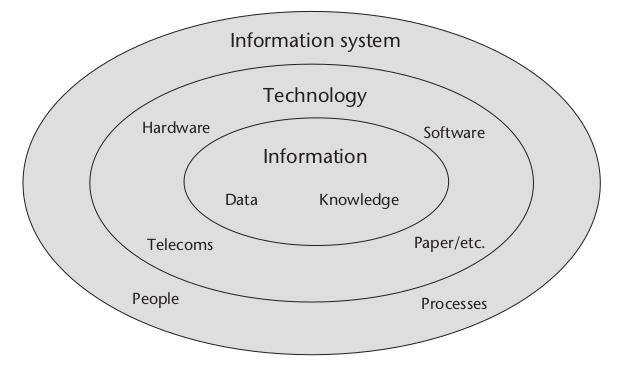
\includegraphics[width=0.8\textwidth]{e-gov-sys-as-info-sys}
	\caption[e-Government systems as information systems]{e-Government systems as information systems}
	\label{fig:e-gov-sys-as-info-sys}
\end{figure}


IT handles data to produce information. E-Government systems are information systems. At their heart lie data and information\footnote{defined as data that has been processed to make it useful to a recipient}. These are handled by digital and sometime non-digital information technologies.

But this does not make a `system'. A system is a collection of elements that works and has purpose. To understand e-government as information system, we must add in some notion of activity and purpose. That can only come if we bring people into the equation. For e-government to be working information system, it must be seen as much more than must the technical elements of IT. Instead, it must be seen to consist of technology plus information plus people who give the system purpose and meaning plus work processes that are undertaken.

Figure {\ref{fig:e-gov-sys-as-info-sys}} shows e-government systems can be described as ‘socio-technical systems’ because they combine both the social – that is, people – and the technical. This is a first indication that, when managing e-government, both social and technical (otherwise known as soft and hard) issues will have to be dealt with.



The model in Figure \ref{fig:e-gov-sys-as-info-sys} is incomplete. eGovernment systems
don’t just float around like satellites in space. Most are embedded within public
sector organizations that provide, for example,
the management systems and the organiza-
tional resources that support e-government.
These organizations also provide things
like the political and cultural milieu
within which e-government operates. Many
e-government systems also reach out to
other groups (citizens, businesses); a few
involve other public agencies. In turn, all
these groups and organizations are themselves embedded in institutional environments: a broader context of laws and values,
economic systems and technological innovations that affects both the agencies/groups
and the systems – including e-government
systems – that serve them.

Full model of e-government must embrace these factors, as shown in Figure \ref{fig:full-model-of-e-gov}.
 
 %%%%%%%%%%%%%%%%%%%%%%%%%
 %						%								
 %		FIGURE			%
 %						%
 %%%%%%%%%%%%%%%%%%%%%%%%%
 \begin{figure}[ht]
 	\centering
 	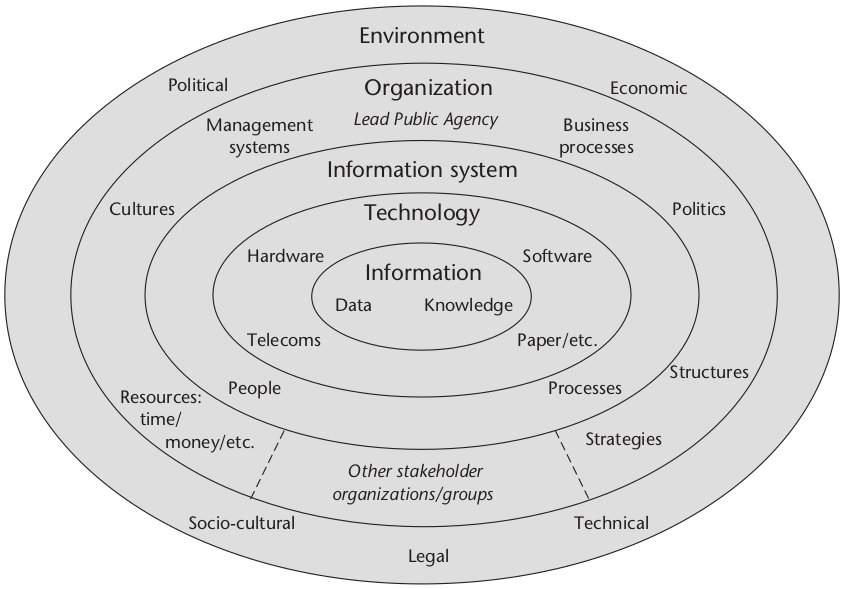
\includegraphics[width=0.8\textwidth]{full-model-of-e-gov}
 	\caption{Full model of e-government systems}
 	\label{fig:full-model-of-e-gov}
 \end{figure}


\begin{framed}
		\begin{nepali}
			\begin{center}
			\noindent Figure \ref{fig:full-model-of-e-gov} मा चित्रण गरिएकाे चित्रलाई 'onion-ring' model पनि भनिन्छ।
		\end{center}	
	\end{nepali}
\end{framed}

\subsection*{The ITPOSMO Checklist}
In fully describing and understanding an
e-government system, we could refer to every
one of the 20 separate factors identified in
Figure \ref{fig:full-model-of-e-gov}. But
that would be complex. Here, we will make more use of a slightly
simpler checklist of key items drawn out
from this `onion-ring' model:

\begin{itemize}
	\item \textbf{I}nformation: The formal information held by the digital system and the informal information used by the people
	involved with the system.
	
	\item \textbf{T}echnology: Mainly focuses on digital IT but can also cover other information	handling technologies such as paper or analogue telephones.
	
	\item \textbf{P}rocesses: The activities undertaken by the relevant stakeholders for whom the
	e-government system operates, both information-related processes and broader business processes.
	
	\item \textbf{O}bjectives and values: Often the most
	important dimension since the objectives
	component covers issues of self-interest
	and organizational politics, and can
	even be seen to incorporate formal organizational strategies; the values component covers culture: what stakeholders feel are the right and wrong ways to do
	things.
	
	\item \textbf{S}taffing and skills: Covers the number of
	staff involved with the e-government
	system, and the competencies of those
	staff and other users.
	
	\item \textbf{M}anagement systems and structures: The
	overall management systems required
	to organize operation and use of the
	e-government system, plus the way
	in which stakeholder agencies/groups
	are structured, both formally and
	informally.
	
	\item \textbf{O}ther resources: Principally, the time
	and money required to implement and
	operate the e-government system.
\end{itemize}

This ITPOSMO checklist can be used
for describing and understanding any
e-government system and stakeholder
organizational context.

In some cases, it may be important to also
describe the wider context, by expanding
the checklist to ITPOSMOO, adding an
eighth dimension:


\begin{itemize}
	\item \textbf{O}utside world: The political, economic,
	socio-cultural, technological and legal
	factors that impinge on the relevant
	e-government stakeholders.
\end{itemize}

\subsection*{The CIPSODA Checklist}
Given that e-government systems are
information systems, we can draw on one
further model/checklist to help us understand e-government. This understands an
e-government application in terms of its
information-related tasks: a process view to
go alongside the structural view offered
above. These tasks are summarized by the
CIPSODA checklist, illustrated in Figure \ref{fig:e-gov-process-view}.

The checklist of tasks can be explained in
some further detail, using the example of
part of an e-tax system:

%%%%%%%%%%%%%%%%%%%%%%%%%
%						%								
%		FIGURE			%
%						%
%%%%%%%%%%%%%%%%%%%%%%%%%
\begin{figure}[ht]
	\centering
	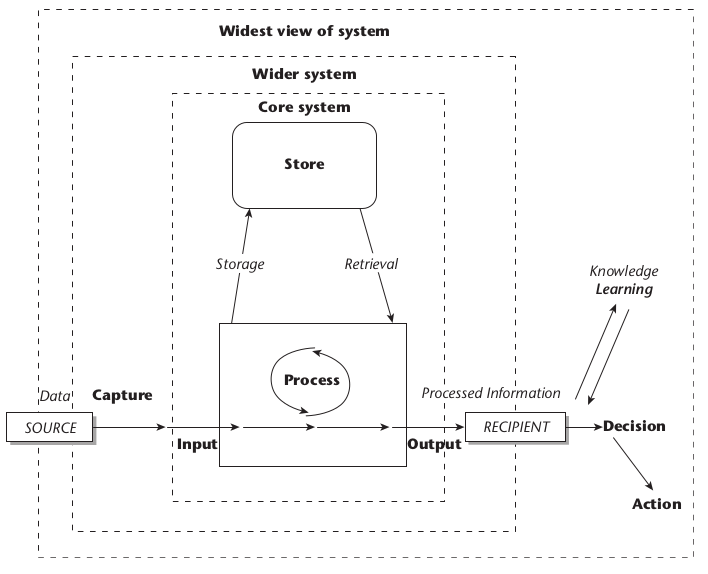
\includegraphics[width=0.8\textwidth]{e-gov-process-view}
	\caption{eGovernment systems as information systems: Process view}
	\label{fig:e-gov-process-view}
\end{figure}

\begin{itemize}
	\item \textbf{C}apture: Gathering the raw data necessary for the e-government system. The
	taxpayer obtains the basic data on their
	various sources of income.
	
	\item \textbf{I}nput: Entering the data onto the system.
	The taxpayer types the data into an
	e-form on the revenue agency’s website.
	
	\item \textbf{P}rocess: Altering the data via calculation,
	classification, selection, and so on. The
	e-tax system uses the different tax rates
	for different income types to calculate
	the total tax owed.
	
	\item \textbf{S}tore: Holding raw and processed data
	on the system. The e-tax system stores all
	details entered and calculated about this
	taxpayer.
	
	\item \textbf{O}utput: Issuing the processed data. The
	total tax calculated is displayed to the
	taxpayer.
	
	\item \textbf{D}ecision: If the processed data is useful
	enough to be seen as information, it is
	used for decision-making. The taxpayer
	determines whether to challenge or
	accept the calculated tax sum.
	
	\item \textbf{A}ction: Implementation of the decision.
	If all is well, the taxpayer authorizes payment of the tax owed.

\end{itemize}
Note there is also an eighth task implicit
within the model: the communication of
data between each of the other tasks.

While Figure \ref{fig:full-model-of-e-gov} uses an information
systems perspective to explain what an
e-government system \textit{is}, Figure \ref{fig:e-gov-process-view} explains
more what an e-government system \textit{does}.


\section{Benefits of e-Government}

\subsection{Benefits to Government}
\subsubsection{Law and Policy Making}
ICTs, especially the internet, enable gathering of model legislations and policies at international and national levels on any subject, and the experience of nations and regions in the implementation of those laws and policies. It is therefore possible to formulate new policies or modify/review existing laws and policies in a quicker time-frame and in a more informed manner.

e-Government, implemented extensively over a period, generated enough data and MIS that enable policy makers in  better decision-making.

The strength of laws and policies depends on how widely they are disseminated. Internet is the best-suited medium for this purpose. In fact, publication of all the Acts, Rules and Regulations on websites and portals is one of the common initiatives undertaken by a majority of the nations leading in the e-Government field.

\subsubsection{Regulation}
The following areas of regulation can immensely benefit from e-Government initiatives:
\begin{multicols}{2}
	\begin{itemize}
		\item Statutory registrations of companies and business under various laws
		\item Taxation
		\item Environmental regulations
		\item Police
		\item Transportation
		\item Healthcare
		\item Education
		\item Food and agriculture
		\item Industry and commerce
	\end{itemize}
\end{multicols}


Benefits in the regulatory areas could be in one or more of the following forms:

\begin{enumerate}
	\item Better compliance due to stringent tracking and monitoring systems
	\item Better revenues
	\item Better coordination between related regulatory agencies (e.g. police and transportation) due to shared databases
	\item More transparency in enforcement of laws
\end{enumerate}

\subsubsection[Electric Service Delivery]{Provision of Services-Electric Service Delivery (ESD)}
Electronic Service Delivery (ESD) is beneficial to the citizens as well as government. Following are the benefits of ESD to the government.

\begin{itemize}
	\item \textit{Better image}: Speed, efficiency, transparency and convenience arising out of ESD enhance the image of government.
	\item \textit{Cost cutting}: The automation process reduces manpower costs, besides costs of accounting, compilation, reporting and review.
\end{itemize}


\subsection{Benefits to Citizens}
The cost citizens has to incur on ascertaining the forms and procedure appropriate to the service needed, travelling to the designated government agency or to an intermediary/agent multiple time are where citizen lose their valuable time and money. By using e-government setup these costs can be reduced or eliminated.
Besides cost reduction, the other benefits to the citizen can be in the form of:

\begin{enumerate}[label=(\alph*)]
	\item increased transparency leading to reduced corruptions.
	\item better planning of personal and professional work arising out of definiteness in dealing with the government.
	\item better quality of life as a result of the use of ICT in areas such as health, education, employment, welfare and finance.
	\item easy access to information on government agencies and programmes.
	\item multiple delivery channels to choose from, thus adding to convenience and
	\item facilities like single-window and Single-Sign-On that remove the complexities of visiting multiple government agencies or websites.
\end{enumerate}


\subsection{Benefits to Business}
\subsubsection{Increased Velocity of Business}
With the digitization of the G2B interface, the velocity of business increases. Ease of filing returns and enhanced speed in securing the various permits and licenses through electronic single windows are examples.

\subsubsection{Ease of Doing Business With Government}
e-procurement provides a convenient Internet-based medium for online registration of suppliers, bidding for works and projects, and tracking the status of their award.


\section{e-Government Stages of Development}
The theoretical progression of e-Government in any country or state is along \textit{four stages} which indicate the extent of benefits that the stakeholders get through the e-Government projects prevalent in that country or state. These are represented schematically in Figure {\ref{fig:e-gov-dev-stages}}.


%%%%%%%%%%%%%%%%%%%%%%%%%
%						%								
%		FIGURE			%
%						%
%%%%%%%%%%%%%%%%%%%%%%%%%
\begin{figure}[ht]
	\centering
	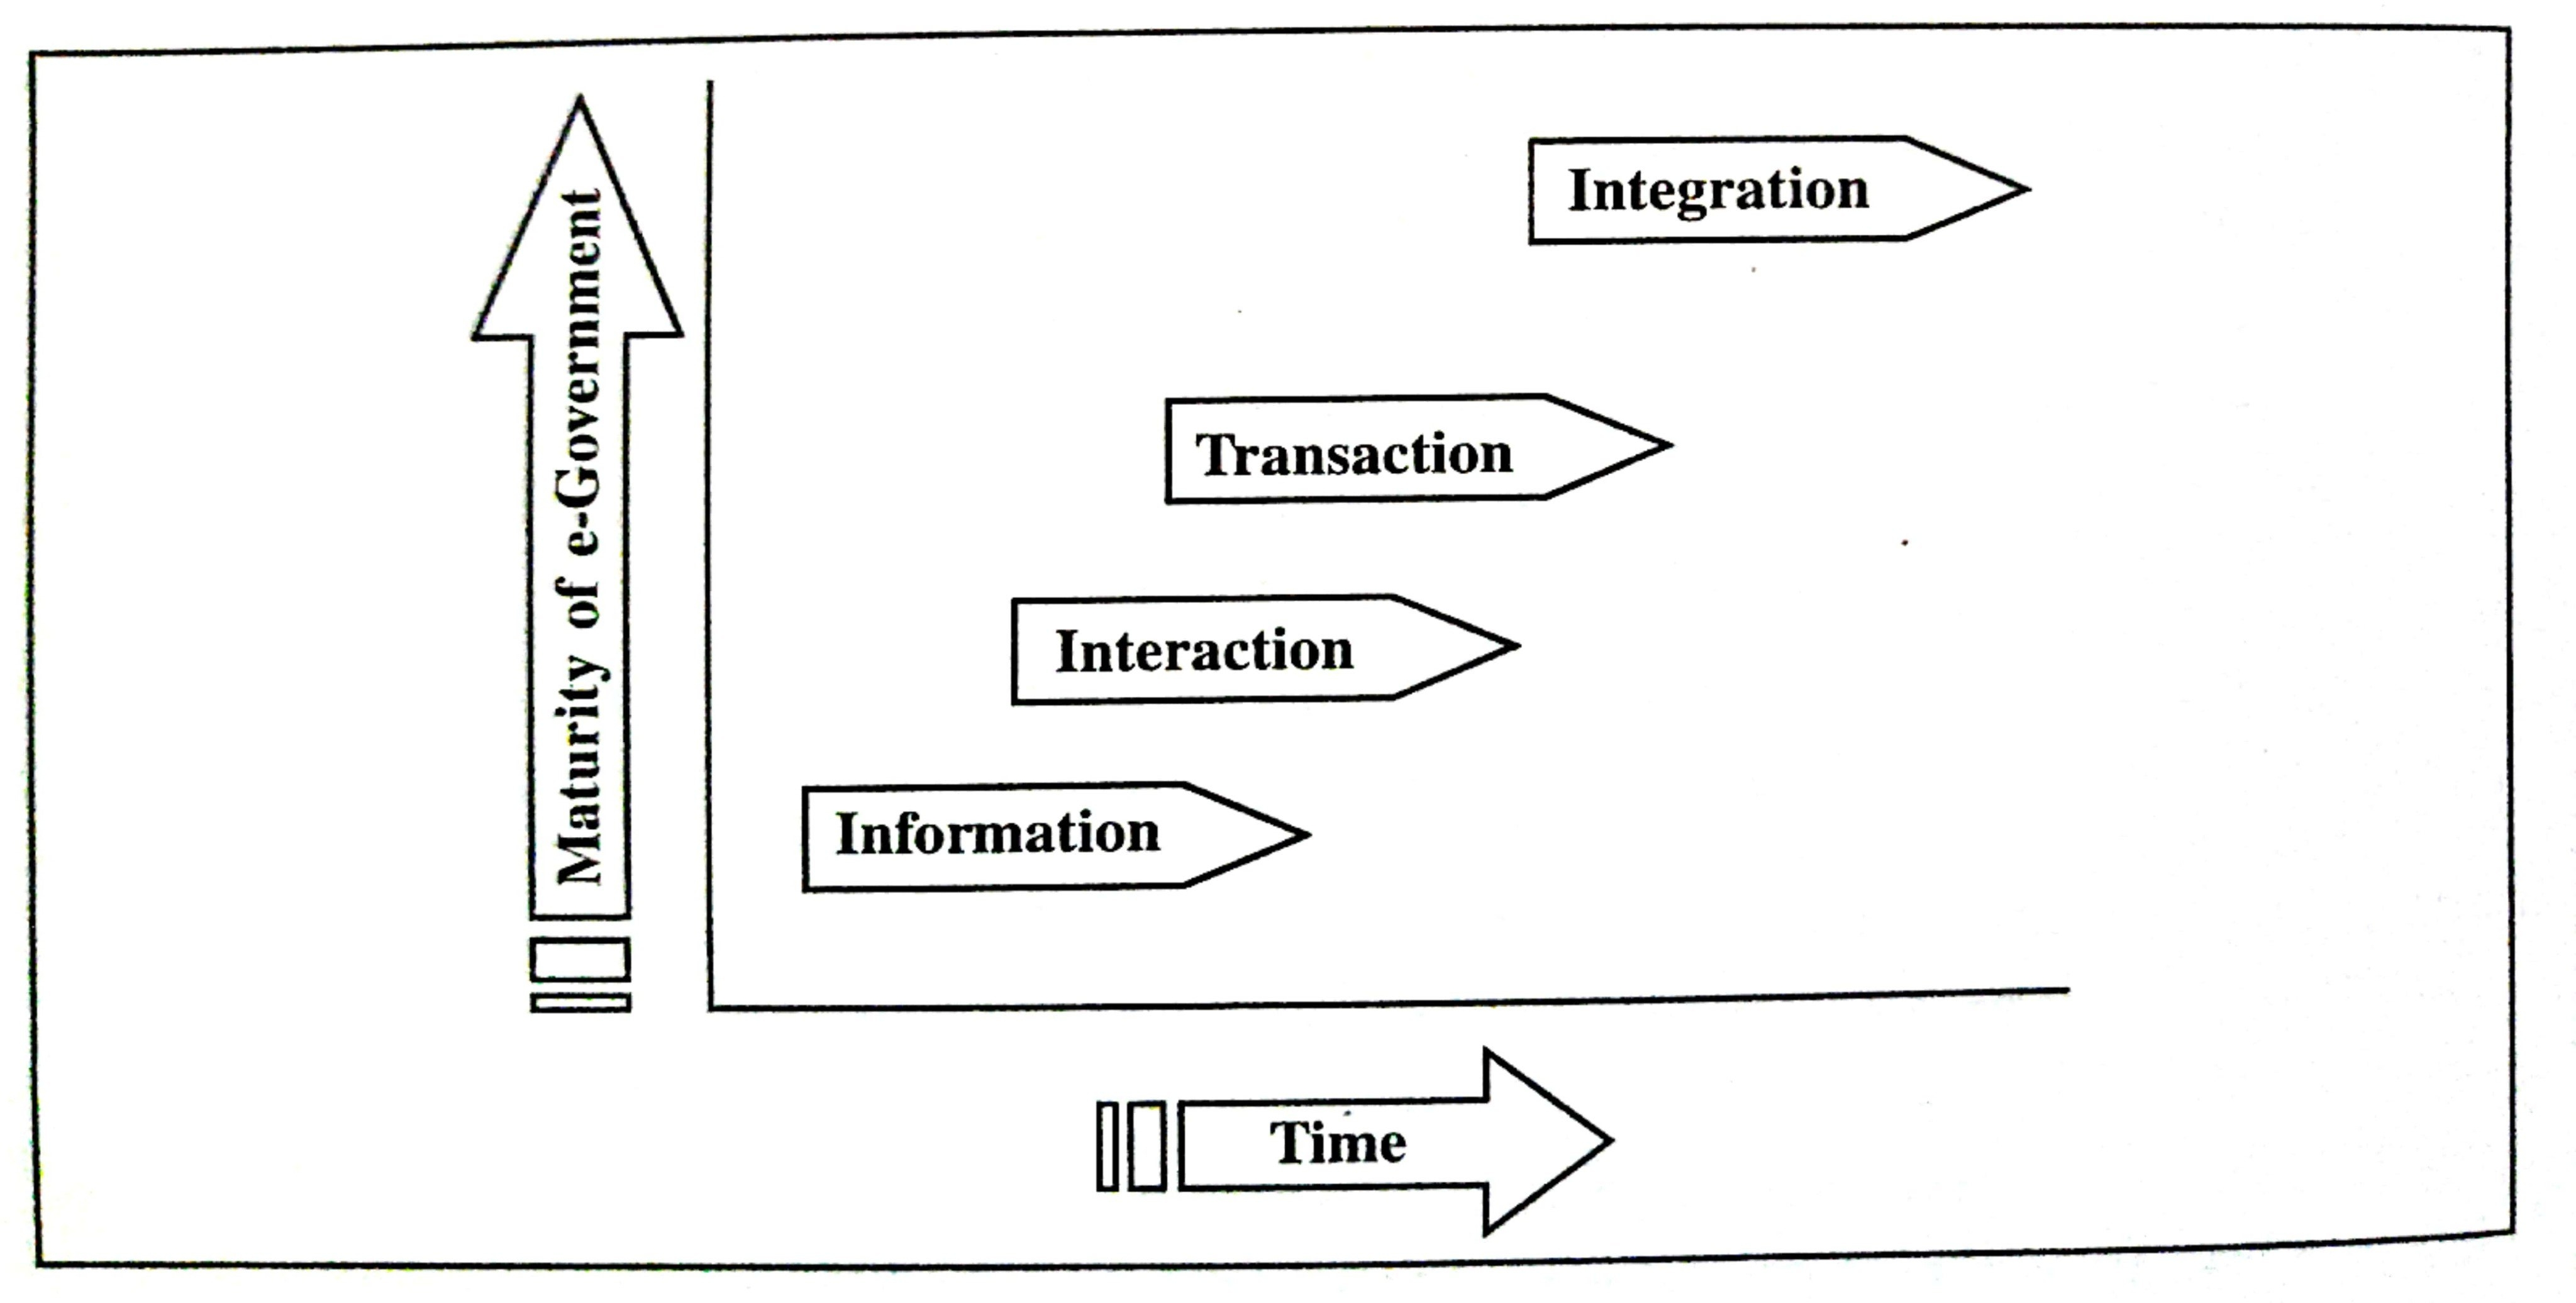
\includegraphics[width=0.8\textwidth]{e-gov-dev-stages}
	\caption{e-Government systems as information systems}
	\label{fig:e-gov-dev-stages}
\end{figure}

\subsection{Information}
This is the initial stage of web presence. A few websites are launched that contain limited and static information, which is updated more frequently with increasing usage and customer pressure. The information may be limited to basic functions, facts and figures and contact details of government departments and agencies. The information stage does not call for any efforts at `Computerization’ of the backend.

\subsection{Interaction}
In this stage, the citizen can \textit{interact} with the government agencies in a ‘one way street’ manner. The citizens can download forms, file forms, returns and complain online, with government agencies. This stage calls for building capacity and systems in the backend government agencies to receive the request send by the
citizen online and to process in sequential and accountable manner. The interactive website reduce the tedium of the citizen partially by enabling them to save at least one step in dealing with government agencies.

\subsection{Transaction}
This is a much more difficult stage to reach. In the transactional stage, the citizens can go through a full cycle of fulfillment of their request. It is a two-way street.  Complete and secure transactions such as online payments for utility bills, taxes, fees, registration, renewals, obtaining permits, licenses and certificates are typical examples of transactions. e-Procurement, Online customs clearance, single window and single-sign-on are more sophisticated examples of this stage. This requires extensive system study, establishing data centers, disaster recovery and management system. The services have to be delivered on a $24\times7$ basis, the services should be citizen centric and should reflect the transformation that is the hallmark of e-government.

\subsection{Integration}
This is yet the Utopian\footnote{An idealistic (bust usually impractical)} stage of e-government. This stage envisages\footnote{Form a mental image of something that is not present} offering government information and services in an integrated manner not only from government view but also from citizen and business side. The key events in the citizen’s life are- birth, admission to school, admission to college/university, employment, housing, marriage, shifting of job/house, medicare, senior citizenship and death. The key events of business are registration of a firm/company, securing all clearances for setting up business/industries, filing of returns, payment of taxes and winding up.


\section{Online Service Delivery and Electronic Service Delivery}
\subsection{Online Service Delivery}
Online service delivery is the system of e-government by providing information and other various services through the means of Internet. Most services can be provided by online and services are available anywhere anytime but only the limitation is lack of availability of Internet to all places and not every citizen are computer-literate. Also, government have to initially invest large budget for establishing, utilizing and securing ICT system for online service delivery.


\subsection{Electronic Service Delivery}
Electronic service delivery means providing the services to citizen and business
electronically without Internet i.\ e.\ Television, Radio, Telephone, SMS system etc.



\newpage\thispagestyle{empty}








